\chapter{Síntese de Voz}

	\subsection{Modelo Massa-Mola Auto Sustentável}:
	A fechadura e abertura da glote num sistema massa mola de apenas um lado

	\[
		P = (1 - \frac{a2}{a1})*(Ps- Pi) + Pi
	\]
		
	
	Versão simplificada da pressão massa mola
	\begin{itemize}
		\item P: Pressão resultante NA GLOTE
		\item a1: Areas de entrada da glote
		\item a2: Areas de saída  da glote
		\item Ps: Pressão subglotica
		\item Pi: Pressão sobre o trato vocal(Pressão input)
	\end{itemize}
	
		No modelo mono massa a1 = a2.No caso em que Pressão na GLOTE,P, seja  igual a pressão  supraglotal, indica que a inércia da coluna de ar acima da glote altera a pressão.
	
	
	\subsection{Synpath}
		O SynPath é um sintetizador computacional, desenvolvido em linguagem Python [13, 20, 28], criado por Lucero~\cite{LuceroZueiro1}. Este software é uma extensão do sintetizador concebido por Fraj[19], incorporando um modelo de vibração para as pregas vocais. O seu propósito é aumentar a fidelidade fisiológica do sintetizador de Fraj e permitir o controle direto dos sons sintetizados em termos de parametrização da laringe. Para se obter um simples controle sobre o sintetizador e facilitar o seu uso para aplicações práticas, é necessário que a representação das pregas vocais seja simples. Além disso, o modelo das pregas vocais deve garantir variações suaves no fluxo gerado na glote. A falta de suavidade gera timbres não naturais e consequentemente a perda da fidelidade fisiológica buscada. Sendo assim, o modelo multi-massa para representação das pregas vocais não pode ser utilizado visto que produz variações não suaves e é um modelo matematicamente muito complexo levando a instabilidades numéricas, afetando o uso para aplicações práticas. O SynPath tomou como base para a representação das pregas vocais o modelo de onda mucosa desenvolvido por Titze [26]. Basicamente, o modelo é um oscilador mono-massa, conforme descrito no Capitulo 3, incorporando a transferência de energia do fluxo de ar para as pregas vocais. Entretanto, o modelo de Titze possui duas restrições, uma que foi solucionada e aplicada no desenvolvimento do SynPath e a outra que ainda não foi solucionada e portanto é também uma restrição do modelo computacional do SynPath. A primeira restrição é que o modelo de Titze foi concebido para o estudo em pequenas oscilações, sendo que para oscilações de maior amplitude, este não é apropriado. Entretanto, esse modelo foi extendido por Lucero [11] para abranger maiores oscilações utilizando um mecanismo limitador de amplitude durante as oscilações [14]. Mesmo com essa extensão para maiores amplitudes, o modelo ainda apresentava uma outra restrição, um atraso pequeno para o deslocamento da onda no canal glotal. A consequência desse atraso é que a pressão limite para que ocorra a vibração se torna independente da frequência de vibração [15]. Porém, sabe-se que um esforço maior é necessário para que tons mais agudos sejam vocalizados, ou seja, a pressão para que se ocorra vibração em frequências maiores(tons maiores) é maior. Essa restrição ainda não foi solucionada tendo em vista a dificuldade de se realizar o supracitado computacionalmente. Mesmo com essa restrição, o modelo de Lucero [11] é o modelo utilizado para
		26
		a representação do caráter oscilatório das pregas vocais no software SynPath, sendo que esta restrição não solucionada não tem forte influência no produto final.
		
	
		\subsubsection{Requisitos Funcionais}
		
		O Synpath é consistido também dos seguintes requisitos funcionais, os requistos funcionais são as funcionalidades que o sistema executará\cite{SWEBOK}
		
		\begin{itemize}
			\item 1 - Validação do Parâmetros passados pelo Usuário, se condizem com restrições do programa.
			\item 2 - Plotar um gráfico inicial do trato vocal de acordo com os parâmetros do usuário.
			\item 3 - Plotar três gráficos referentes as propriedades da voz simuladas com os parâmetros fornecidos pelo usuário. – O primeiro gráfico refere-se às posições adotadas pelas cordas vocais, a área da glótis, ao fluxo de ar nessa área e às características desse fluxo. – O segundo gráfico refere-se às características do som gerado pela simulação física do aparato fonador pelo programa. – O terceiro gráfico refere-se ao espectro de frequência do som gerado e do fluxo da glótis.
			\item 4 - Gerar um arquivo de texo com as características de voz gerada, frequencia,amplitude, ruído da voz, entre outros
			\item 5 Gerar um arquivo de som de voz simulada.
		\end{itemize}
		
		\subsubsection{Requisito Não-Funcionais}
		
		O Synpath consiste também dos seguintes requisitos não funcionais, requisitos não funcionais são requisitos são parametros de qualidade, requisitos que limitam as funcionalidades do sistema\cite{SWEBOK}.
		
		\begin{itemize}
			\item 1 - O Sistema deve produzir os gráficos que os requisitos funcionais delimitaram em um intervalo de 1(um) minuto. 
			\item 2  - Após gerar os gráficos e os exibi-los o arquivo texto e o arquivo de audio deverão ser exibidos
			\item 3 - Para que o sistema esteja funcional é necessário ter instalado os pacotes: MatPlotLib e NumPY
			\item 4 - O sistema deve ser executado em plataformas de um sistema operacionais como Windows, Linux ou MacOs, Versões recentes de acordo com a data desse documento. 
			
		\end{itemize}
		
	
	
	
	
	\subsection{HMMs}
		Minera-se de várias partituras musicais para treino. Os dados minerados dessas músicas são fonemas, altura, intensidade e os intervalos, isto é relação com outras notas.Esses dados são convertidos e mapeados em "labels" dependentes de contexto~\cite{DegottexNada}.Após isso as HMM's são treinados através dos dados de treinamento usando o algoritmo EM.\cite{GudnasonNada}. Após isso ocorre a fase de sintesis, usa-se outra partitura para ser convertida em "labels" dependentes de contexto e estima-se quais "labels" preprocessadas são correspondentes.\cite{TakashiNose}
	
		\subsection{MHRSMM}
		Uma variação HSMM. Modelo de multipla regressão HSMM.
		Parametros importantes são μi e mi dos outputs pdfs
		
		\[ \mu_i = H_bi \xi \] 
		\[	m_i   = H_pi \xi  \]
		\[ \xi   = [1,v_1,v_2,...,v_L]^T \]	
		\[ \xi   = [1,v^T]^T	\]	
		
		Onde L é a dimensão do vetor de estilo e vi  é  a intensidade do  enésimo estilo de canto.
		
		Um exemplo de um vetor de estilos de canto de tamanho L =  2 e L = 3.
		
		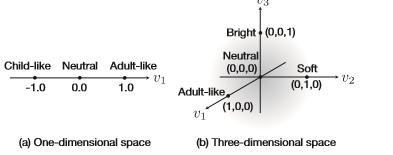
\includegraphics{exemploHMM.png}
		
		\subsubsection{Controle do Sintentisador de voz cantada baseado em MRHSMM}
		
		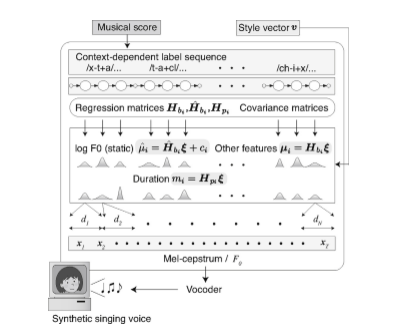
\includegraphics{esquemaHMM.png}
		
		Durante a fase de síntese o usuário do programa adiciona vetores de estilos de acorodo com a intenção e a expressividade pretendida.
		Parametros de output como duração são gerados pelos vetores de estilos dados e matrizes de regressões treinadas usando MRHSMMs
		
		Resultado de todo esse processo é um sequência HSMM usando parametros de geração de fala
		
		MRHSMM possui uma dificuldade de gerar contorno F0 que acompanhe o contexto de mudança de altura das notas o author TAKASHI NOSE, propõe um treinamento de HSMM e HMM nos parametros 
		
	
	\subsection{FrameWorks Sintetisador de Voz}
	
		Frame Work de um Sistema Sintetisador de Voz:
		
		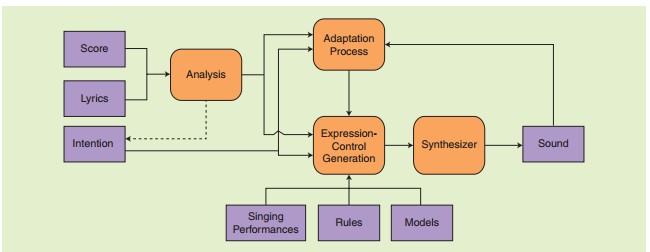
\includegraphics{frameWork.png}
		
		\subsubsection{Input}
		Consiste da partitura, letra e emoção.
		o input é analisado e derivado em uma transcrição fonética, alinhamento com a performance alvo ou dados contextuais.\cite{FrameWork}\linebreak
		
		\subsubsection{Expressão}
		Expressão músical é um conceito intuitivo porém dificil de se definir. A expressão é chave na percepção da qualidade e naturalidade musical.
		No caso da voz cantada implica-se usar vários outros parametro além de frequencia e amplitude. Psicológicamente contorno do timbre, vibrato, tremolo, timing fonético.\cite{FrameWork}\linebreak
	
	
	\subsection{Envoltoria F0}
	
	Envoltórias F0 são usadas para expressar informação linguistica, para-linguística e não-linguistica.\cite{SaitouF0}
	\linebreak
	
	As Envoltória F0 apresentam três (3) características importantes que fazem diferenciar uma voz falada a uma voz cantada.\cite{SaitouNada}
	\linebreak
	\begin{itemize}
		\item 1 - O alcance dinâmico de uma envoltória F0 é mais largo que o de uma voz falada
		\item 2 - A envoltória F0 corresponde e tende a se manter estável em uma nota. A mudança de nota de uma envoltória F0 corresponde a melodia da música
		\item 3 - Existem muita flutuações f0 que são apenas observadas em apenas vozes cantadas
	\end{itemize}
	
	
	\subsection{Sintese de Voz em Mandarím}
		Utiliza-se a técnica HNM para a sintese da voz cantada em mandarím. HNM significa , "harmonic plus noise model".
		O modelo HNM divide o espectro de um sinal em dois(2) com larguras não iguais para modelagem melhor do espectro.\cite{LinRobos}
	